\section{Introduction}

This work focuses on creating and testing valid trajectories for high degree of freedom (DOF), high-gain, position controlled mechanisms that results in the desired end-effector velocity.  Throwing and hitting are examples of end-effector velocity control.  The goal is to have the end-effector moving at a specific rate in a specific direction.  It is also a task that demands whole-body coordination.  When the arm moves quickly, as in the case of pitching, such upper-body motions, if not coordinated with the lower-body, can cause the humanoid to lose balance.  The overarching goal of this work is to create stable whole-body motions that reliably moves the end-effector at the desired velocity while retaining stability.  Fig.~\ref{fig:hubothrow} shows under arm throwing using a trajectory generated from motion capture data, a crucial step towards our overarching goal.
The focus of this work is to compare and contrast three methods of creating full body throwing motions for high gain position controlled robots.






\begin{figure}[t!]%[thpb]
  \centering
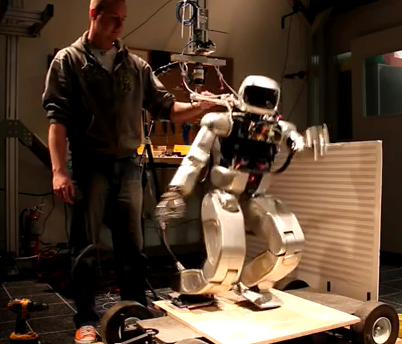
\includegraphics[width=1.0\columnwidth]{./pix/huboThrow.png}
  \caption{Jaemi Hubo (Hubo KHR-4) demonstrating under arm throwing using a trajectory generated from motion capture data.  This shows a crucial step towards our overarching goal of creating a full body, human-like, stable, motion for throwing.}
  \label{fig:hubothrow}
\end{figure}





Humanoid robot is designed to be like a human. They will play soccer as well as giving assistant to people in various situations. The better humanoid can learn from human, the broader territory they have and less artificial they will be. Since we ask the humanoid to throw baseball, our aim is to make it achieve the throwing goal with high human-likeness. In case of this complicated motion, conversional method used for designing the motion such as formulating analytics equations becomes difficult to apply. Adoption of pre-recorded human motion from motion capture system for designing humanoid motion proposes a promising teaching method. Starting from recording human throwing motion, we map the recorded data to the humanoid preserving important human-like characteristics while making sure the throwing goal is achieved.
----describe our approach----

\section{Related Word}
Motion capture systems are increasingly developed and used as important tool in sports training and robotics to generate human-like motion.  There exist enormous robotics researches that reply on motion capture data.  From the sport training perspective, the motion capture system is utilized for example to monitor the movement and reconstruct the movement on a synthetic model. [mirabella]  The focus is on kinematics analysis to improve and transmitting skill in a sport [1][2][3][4]. The key research area in robotics is more of retargeting and execution on the robot than kinematics analysis of the motion data.    
Various approaches for generation of human-like motion for humanoid robots were proposed [qiang][pollard][stefan]. Most of the approaches use 3D marker positions as the starting point of data collection. Stefan et al attempt to use an intermediate model (Master Motor Map) to decouple motion capture data from further post-processing tasks. However this added in another conversion to the overall process which causes data lose. On the other hand, the motion capture system we adopted auto-generates a lower DoF skeleton from the 3D marker clouds. This makes the data collected closer to what we want, and can be seen as a non-physical intermediate model which converts high DoF human motion to lower DoF skeleton motion generated by motion capture system. 
As many of the mentioned researches above are done in case of relatively slow motion, the high-speed throwing motion which requires high dynamic stability becomes a main concern. The ground contact constraints proposed in [qiang] points out the key issue in the dynamic stability. ---how we solve the dynamic stability issue-----   
